% !TeX root = ../main.tex

\chapter{Multiple resource NOMA systems}
\label{ch:multi-resource}
In this chapter, we extend single-resource PD-NOMA to a multiple-resource system, where several shared-resources are used to improve multiuser separation ability. 
Since single-resource PD-NOMA mainly relies on received-power differences, the multiple-resource model allows the BS to further exploit resource-domain channel-vector information. 
For multi-resource PD-NOMA, MMSE-SIC detection is adopted, post-SINR ordering and amplitude-based ordering are considered as two detection-ordering methods, and the performance is compared with HDS-CDMA with ML detection~\cite{lin2023gdma}.

\section{Multi-resource PD-NOMA system model}

Multi-resource PD-NOMA refers to an architecture in which each user can transmit over multiple shared resources. At one symbol time, the received vector is
\begin{equation}
    \bm{y} = \bm{H}\bm{x} + \bm{n},
    \label{eq:multi resource model}
\end{equation}
where $\bm{y}\in\mathbb{C}^{R\times 1}$ are the received signals over $R$ resources, $\bm{x}\in\mathbb{C}^{U\times 1}$ are the transmitted signals of $U$ users and $\bm{n}\in\mathbb{C}^{R\times 1}$ denotes complex AWGN. 
The channel matrix $\bm{H}\in\mathbb{C}^{R\times U}$ is 
\begin{equation}
    \bm{H}=
    \begin{bmatrix}
    \sqrt{P_1\beta_1}h_{1,1} & \sqrt{P_2\beta_2}h_{1,2} & \cdots & \sqrt{P_U\beta_U}h_{1,U}\\
    \sqrt{P_1\beta_1}h_{2,1} & \sqrt{P_2\beta_2}h_{2,2} & \cdots & \sqrt{P_U\beta_U}h_{2,U}\\
    \vdots & \vdots & \ddots & \vdots\\
    \sqrt{P_1\beta_1}h_{R,1} & \sqrt{P_2\beta_2}h_{R,2} & \cdots & \sqrt{P_U\beta_U}h_{R,U}
    \end{bmatrix}.
\end{equation}
The $k$th column $\bm{h}_k$ represents the resource-domain channel vector of user $k$.
For the representative two-resource and three-user case, the model is
\begin{equation}
    \begin{bmatrix}y_A\\y_B\end{bmatrix}
    =
    \begin{bmatrix}
    h_{A,1} & h_{A,2} & h_{A,3}\\
    h_{B,1} & h_{B,2} & h_{B,3}
    \end{bmatrix}
    \begin{bmatrix}x_1\\x_2\\x_3\end{bmatrix}
    +
    \begin{bmatrix}n_A\\n_B\end{bmatrix},
\end{equation}
where the large-scale fading and transmit-power factors are absorbed into each $h_{r,k}$.

We employ MMSE-SIC detection for \eqref{eq:multi resource model}. The resulting filter structure is similar to those widely used in multi-antenna systems~\cite{endo2012uplink,li2013advanced} and pattern division multiple access (PDMA) receivers~\cite{kong2016multiuser}. 
In multi-antenna reception, user separation mainly comes from spatial observations, while in PDMA it is further assisted by user-specific pattern mapping across resources. 
In contrast, the considered multi-resource PD-NOMA system does not adopt sparse signatures or pattern design\cite{mohammadkarimi2018signature}; instead, it relies on the channel vectors across shared resources to improve user separation reliability and overall performance. 
%Hence, our formulation should be interpreted as a resource-domain extension of PD-NOMA.


\section{MMSE-SIC Detection}
The MMSE-SIC receiver provides a low-complexity alternative to joint ML/MAP detection \cite{zanella2005mmse} by applying a linear MMSE filter and successively detecting and cancelling users.
The main quantities needed after filtering are the desired effective channel gain, the residual interference-plus-noise variance, the LLR, and the soft estimate used for cancellation.
For the multi-resource model of \eqref{eq:multi resource model}, 
consider user $k$ be detected. The MMSE filter is designed by following \cite[Eqs. (6), (7)]{kong2016multiuser} with the coefficient
\begin{equation}
\label{eq:coefficient}
    \bm{w}_k^H
    =
    \bm{h}_k^H
    \left(
    \bm{H}\bm{H}^H + 2\sigma^2\bm{I}
    \right)^{-1},
\end{equation}
The filter output of user $k$ can be formulated as
\begin{equation}
    \label{eq:filter output}
    z_k
    =
    \bm{w}_k^H \bm{y}
    =
    \bm{w}_k^H \bm{h}_k x_k
    +
    \sum_{j\neq k}\bm{w}_k^H \bm{h}_j x_j
    +
    \bm{w}_k^H \bm{n}.
\end{equation}
In \eqref{eq:filter output}, we define the effective channel gain:
\begin{equation}
    a_k=\bm{w}_k^H\bm{h}_k,
\end{equation}
and the effective residual interference-plus-noise variance:
\begin{equation}
	\label{eq:effective noise}
    \sigma_{k,\rm eff}^2
    =
    \sum_{j\neq k}
    |\bm{w}_k^H \bm{h}_j|^2
    +
    2\sigma^2 \|\bm{w}_k^H \|^2.
\end{equation}

\subsection{Detection Ordering}
\label{sec:MMSE SIC detection order}
To determine  successive detection orders in the SIC process, two ordering strategies are considered. The first is post-SINR ordering \cite{li2013advanced}. The post-filtering SINR of user \(k\) is
\begin{equation}
    \gamma^{\mathrm{post}}_k
    =
    \frac{\abs{\bm{w}_k^H\bm{h}_k}^2}
    {\sum_{j\ne k}\abs{\bm{w}_k^H\bm{h}_j}^2+2\sigma^2\norm{\bm{w}_k}^2}.
    \label{eq:post-sinr}
\end{equation}
The receiver detects the user with the largest post-SINR first. This criterion uses both the magnitude and phase of the channel information, and it reflects the actual quality of each user after MMSE filtering, which are generally preferred in reducing SIC error propagation.

The second strategy is amplitude-based ordering. Users are sorted according to a channel magnitude or received-power metric such as
\begin{equation}
    \gamma^{\mathrm{amp}}_k=\norm{\bm{h}_k}^2.
\end{equation}
This ordering is simpler because it relies only on channel magnitudes, but ignores how MMSE filtering suppresses multiuser interference.
After determining the SIC orders and then re-numbering the user indexes, we assume 
\begin{equation}
    \label{eq:detection order}
    \gamma_1 \geq \ldots \geq \gamma_U
\end{equation}
for simplicity.
This renumbering is applied for either one of the ordering strategies and simplifies the superscript.


\begin{comment}
\subsection{SIC Procedure}
After the order is chosen, users are renumbered as $1,2,\ldots,U$. The SIC procedure is similar to section ~\ref{sec:Detection principle for PD NOMA : soft SIC}. 
At the ${(i+1)}^{th}$ SIC stage, the SIC detector performs the subtraction by setting
\begin{equation}
    \label{eq:soft cancellation}
    \bm{y}_{(i+1)} = \bm{y}_{(i)} - \bm{h}_i \hat{s}_i
\end{equation}
with $\bm{y}_{(1)} = \bm{y}$, where $\bm{y}_{(i)}$ denotes the residual vector at stage $i$.
The corresponding column of $\bm{H}$ in \eqref{eq:multi resource model} is then removed by setting
\begin{equation}
    \bm{H}_{(i+1)}=[\bm{h}_{i+1},\ldots,\bm{h}_U]
\end{equation}
where $\bm{H}_{(1)} = \bm{H}$.
The process then goes back to re-calculate the coefficient $\bm{w}_{i+1}^H$ by using \eqref{eq:coefficient}, the corresponding filter output and the effective variance of the residual interferences and noise can be derived as 
\begin{equation}
    \label{eq:filter output stage i}
    z_{i}
    =
    \bm{w}_{i}^H \bm{y}_{(i)}
    =
    \bm{w}_{i}^H \bm{h}_{i} x_{i}
    +
    \sum_{j > i} \bm{w}_{i}^H \bm{h}_j x_j
    +
    \bm{w}_{i}^H \bm{n}.
\end{equation}
\begin{equation}
	\label{eq:effective noise stage i}
    \sigma_{i,\rm eff}^2
    =
    \sum_{j > i}
    |\bm{w}_{i}^H \bm{h}_j|^2
    +
    2\sigma^2 \|\bm{w}_{i}^H \|^2.
\end{equation}
For a general modulation alphabet $\mathcal{S}$, the LLR of the $q$th bit\cite{shapiro2005soft} is calculated by
\begin{equation}
    L_{x_i,q}
    =
    \log
    \frac{
    \sum\limits_{s\in\mathcal{S}_{q,+}}
    \exp\left(-\frac{\abs{z_i-a_i s}^2}{\sigma^2_{i,\mathrm{eff}}}\right)}
    {\sum\limits_{s\in\mathcal{S}_{q,-}}
    \exp\left(-\frac{\abs{z_i-a_i s}^2}{\sigma^2_{i,\mathrm{eff}}}\right)},
    \label{eq:mmse-sic-general-llr}
\end{equation}
where $\mathcal{S}_{q,+}$ and $\mathcal{S}_{q,-}$ are the subsets of constellation symbols whose $q$th bit is mapped to $+1$ and $-1$, respectively. 
The corresponding soft estimate \cite{shapiro2005soft}
\begin{equation}
    \hat{s}_i
    =
    \mathbb{E}[x_i|z_i]
    \approx
    \frac{
    \sum\limits_{s\in\mathcal{S}} s
    \exp\left(-\frac{\abs{z_i-a_i s}^2}{\sigma^2_{i,\mathrm{eff}}}\right)}
    {
    \sum\limits_{s\in\mathcal{S}}
    \exp\left(-\frac{\abs{z_i-a_i s}^2}{\sigma^2_{i,\mathrm{eff}}}\right)}.
    \label{eq:mmse-sic-general-soft-estimate}
\end{equation}
For BPSK modulation, $\mathcal{S}=\{+1,-1\}$, and \eqref{eq:mmse-sic-general-llr} becomes
\begin{equation}
    L_i
    =
    \frac{4\Re\{a_i^* z_i\}}{\sigma^2_{i,\mathrm{eff}}}.
\end{equation}


If $\hat{s}_i$ is unreliable, the subtraction leaves a cancellation residual in $\bm{y}^{(i+1)}$. This residual is one of the main sources of error propagation in MMSE-SIC, and it motivates the variance-aware coded receiver developed in Chapter~\ref{ch:coded}.
\end{comment}


\subsection{SIC Procedure}

After the order is decided, users are renumbered as $1,2,\ldots,U$. At stage $i$, the residual vector is $\bm{y}_{(i)}$ and the corresponding channel matrix is
\begin{equation}
    \label{eq:downsized channel matrix}
    \bm{H}_{(i)}=[\bm{h}_i,\bm{h}_{i+1},\ldots,\bm{h}_U].
\end{equation}
The MMSE filter output and the effective variance of the residual interferences and noise can be derived as 
\begin{equation}
    \label{eq:filter output stage i}
    z_{i}
    =
    \bm{w}_{i}^H \bm{y}_{(i)}
    =
    \bm{w}_{i}^H \bm{h}_{i} x_{i}
    +
    \sum_{j > i} \bm{w}_{i}^H \bm{h}_j x_j
    +
    \bm{w}_{i}^H \bm{n}.
\end{equation}
\begin{equation}
	\label{eq:effective noise stage i}
    \sigma_{i,\rm eff}^2
    =
    \sum_{j > i}
    |\bm{w}_{i}^H \bm{h}_j|^2
    +
    2\sigma^2 \|\bm{w}_{i}^H \|^2.
\end{equation}
After MMSE filtering, the output can be approximated as an equivalent scalar channel
\begin{equation}
    z_i = a_i x_i+\eta_i,
    \qquad
    a_i=\bm{w}_i^H\bm{h}_i,
    \qquad
    \eta_i\sim\mathcal{CN}(0,\sigma^2_{i,\mathrm{eff}}).
    \label{eq:mmse-sic-equivalent-scalar-channel}
\end{equation}
For a general bit-labeled constellation alphabet $\mathcal{S}$, let
$b_m(s)\in\{0,1\}$ denote the $m$th label bit of symbol $s$, and define
\begin{equation}
    \mathcal{S}_{m,b}
    =
    \{s\in\mathcal{S}: b_m(s)=b\},
    \qquad b\in\{0,1\}.
\end{equation}
In this chapter, the transmitted coded bits are assumed to be independent and equally probable. Therefore, the prior term cancels in the likelihood function. Under the scalar Gaussian approximation in \eqref{eq:mmse-sic-equivalent-scalar-channel}, the standard likelihood-marginalization form of the soft-output demapper~\cite{shapiro2005soft} gives the detector LLR of the $m$th bit as
\begin{equation}
    L_{x_i,m}
    =
    \log
    \frac{
    \sum\limits_{s\in\mathcal{S}_{m,0}}
    \exp\left(-\frac{\abs{z_i-a_i s}^2}{\sigma^2_{i,\mathrm{eff}}}\right)}
    {\sum\limits_{s\in\mathcal{S}_{m,1}}
    \exp\left(-\frac{\abs{z_i-a_i s}^2}{\sigma^2_{i,\mathrm{eff}}}\right)},
    \label{eq:mmse-sic-general-llr}
\end{equation}
For BPSK modulation, $\mathcal{S}=\{+1,-1\}$ with $0\mapsto +1$ and $1\mapsto -1$, and \eqref{eq:mmse-sic-general-llr} becomes
\begin{equation}
    L_{x_i}
    =
    \frac{4\Re\{a_i^* z_i\}}{\sigma^2_{i,\mathrm{eff}}}.
\end{equation}
The corresponding soft symbol estimate is the posterior mean obtained from the same equally likely symbol prior~\cite{shapiro2005soft}:
\begin{equation}
    \hat{s}_i
    =
    \mathbb{E}[x_i|z_i]
    =
    \frac{
    \sum\limits_{s\in\mathcal{S}} s
    \exp\left(-\frac{\abs{z_i-a_i s}^2}{\sigma^2_{i,\mathrm{eff}}}\right)}
    {
    \sum\limits_{s\in\mathcal{S}}
    \exp\left(-\frac{\abs{z_i-a_i s}^2}{\sigma^2_{i,\mathrm{eff}}}\right)}.
    \label{eq:mmse-sic-general-soft-estimate}
\end{equation}
This posterior mean reduces to

\begin{equation}
\hat{s}_i=\tanh(L_{x_i}/2)
\end{equation}
if BPSK modulation is used. 
The expression in \eqref{eq:mmse-sic-general-soft-estimate} is therefore a detector-output soft estimate for the uncoded receiver when all transmitted bits are equally likely. 
The soft estimate is then subtracted from the received vector:
\begin{equation}
    \bm{y}_{(i+1)}=\bm{y}_{(i)}-\bm{h}_i\hat{s}_i .
\end{equation}
The process then goes back to re-calculate the coefficient $\bm{w}_{i+1}^H$ by using \eqref{eq:coefficient} with $\bm{H}_{(i+1)}$. The LLR of $x_{i+1}$ and its soft estimate $\hat{s}_{i+1}$ can also be obtained by \eqref{eq:mmse-sic-general-llr} and \eqref{eq:mmse-sic-general-soft-estimate}. This procedure is repeated until all users are detected.

If $\hat{s}_i$ is unreliable, the subtraction leaves a residual of cancellation  in $\bm{y}_{(i+1)}$. This residual is the main source of error propagation in MMSE-SIC, and motivates the variance-aware coded receiver discussed in Chapter~\ref{ch:coded}.

\section{Uncoded Simulation Results}

The main uncoded multi-resource setting uses BPSK transmission, $R=2$ resources, $U=3$ users, independent Rayleigh flat fading, and perfect CSI are assumed. The MMSE-SIC detector is compared with HDS-CDMA with ML detection\cite{lin2023gdma}. We consider two large-scale fading cases: $(\beta_1,\beta_2,\beta_3)=(1,0.1,0.01)$ and $(\beta_1,\beta_2,\beta_3)=(1,1,1).$
$\bar{E}_b$ in the simulations represent the average transmit energy per bit per user, normalized by the number of resources.


\begin{figure}[htbp]
    \centering
    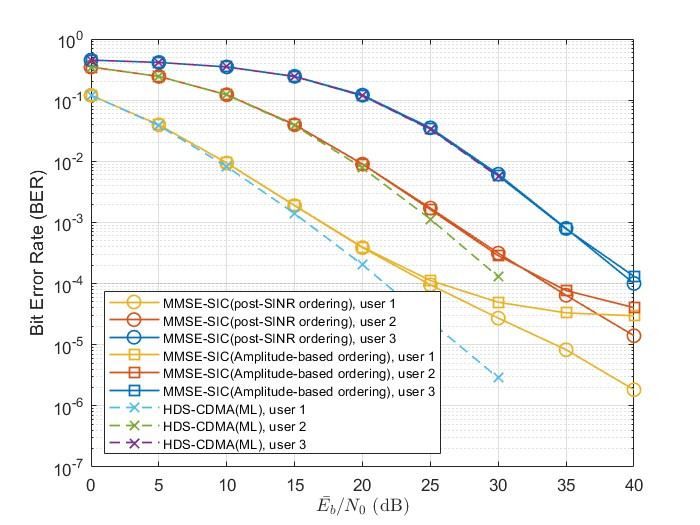
\includegraphics[width=0.9\linewidth]{figures/Chapter3/multi_resource_beta0.1.jpg}
    \caption{Multi-resource system. BER of MMSE-SIC and HDS-CDMA with ML detection with $R=2$, $U=3$ and $(\beta_1, \beta_2, \beta_3) = (1,0.1,0.01)$.}
    \label{fig:multi-resource-beta0-1}
\end{figure}
\begin{figure}[htbp]
    \centering
    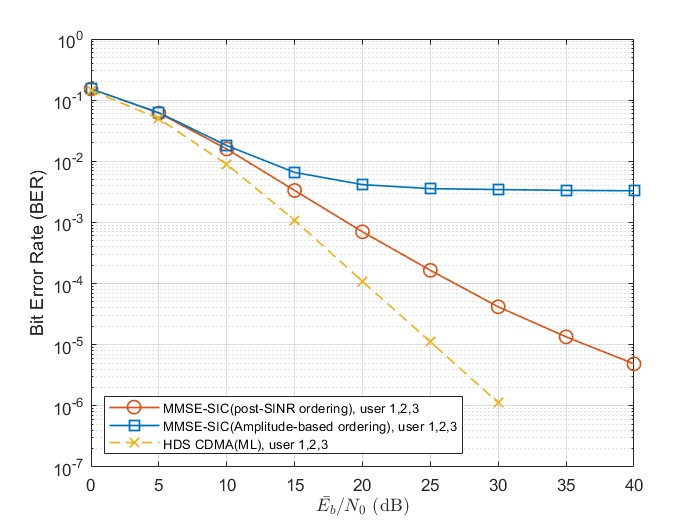
\includegraphics[width=0.9\linewidth]{figures/Chapter3/multi_resource_beta1.jpg}
    \caption{Multi-resource system. BER of MMSE-SIC and HDS-CDMA with ML detection with $R=2$, $U=3$ and $(\beta_1, \beta_2, \beta_3) = (1,1,1)$.}
    \label{fig:multi-resource-beta1}
\end{figure}

The results in figure.~\ref{fig:multi-resource-beta0-1} and \ref{fig:multi-resource-beta1} show that HDS-CDMA with ML detection achieves better uncoded BER than MMSE-SIC in both large-scale fading cases. For the unequal-$\beta_k$ case in figure.~\ref{fig:multi-resource-beta0-1}, HDS-CDMA performs about $3$ dB better than MMSE-SIC at $\mathrm{BER}=10^{-4}$ for user 1. For the equal-$\beta_k$ case in figure.~\ref{fig:multi-resource-beta1}, HDS-CDMA performs about $7$ dB better than MMSE-SIC at $\mathrm{BER}=10^{-4}$. 
Therefore, the performance loss of MMSE-SIC is much more significant when the users have similar average received powers.

The smaller BER gap of two detector in the unequal-fading case is caused by the large-scale fading disparity. Since the users have clearly separated average received powers, the first SIC stage is more reliable and the cancellation error is less likely to dominate the following stages. 
In particular, for the user with the smallest average received power, MMSE-SIC is close to HDS-CDMA within the simulated SNR range. 

The detection ordering comparison further explains the behavior of MMSE-SIC. In the unequal-$\beta_k$ case, amplitude-based ordering only causes a slight degradation around $25$ dB for user 1. In the equal-$\beta_k$ case, however, amplitude-based ordering degrades heavily.

These results indicate that multi-resource PD-NOMA improves user separation compared with single-resource soft SIC, but HDS-CDMA with ML detection remains the stronger uncoded benchmark. The residual performance gap thus motivates the coded system considered in the next chapter.

\begin{comment}
Chapter~\ref{ch:coded} introduces channel coding and iterative detection and decoder (IDD) so that the reliability of the decoder can be used to reduce the propagation of SIC errors.
\end{comment}


